% !TEX program = xelatex
% !TEX encoding = UTF-8 Unicode
% !TEX spellcheck = de_DE

% --------------------------------------------------------------------------- %
% Poster template for Institute of Telematics.      						  %
% --------------------------------------------------------------------------- %
% Created with Brian Amberg's LaTeX Poster Template. Please refer for the     %
% attached README.md file for the details how to compile.				      %
% --------------------------------------------------------------------------- %
% $LastChangedDate:: 2017-08-03 18:00:00 +0200 (V, 12 szept. 2017)          $ %
% $LastChangedRevision:: 129                                                $ %
% $LastChangedBy:: allner                                                   $ %
% $Id:: poster.tex 128 2011-09-11 08:57:12Z rlegendi                        $ %
% --------------------------------------------------------------------------- %


\documentclass[a0paper,portrait]{baposter}

\usepackage[utf8]{inputenc}
\usepackage{relsize}		% For \smaller
\usepackage{url}			% For \url
\usepackage{epstopdf}	% Included EPS files automatically converted to PDF to include with pdflatex
\usepackage{verbatimbox}
\usepackage{enumitem}
\usepackage{wrapfig}
%\usepackage{natbib}
\usepackage{setspace}
\usepackage{uzlcolor}
\usepackage[ngerman]{babel}
\usepackage{blindtext}
\usepackage{cite}



%%% Myriad Pro Font - %%%%%%%%%%%%%%%%%%%%%%%%%%%%%%%%%%%%%%%%%%%%%%%%%%%%%%%%%
\usepackage{fontspec}
\defaultfontfeatures{Mapping=tex-text,Scale=MatchLowercase}
\setmonofont{Myriad Pro}
\setmainfont[
BoldFont={Myriad Pro}, 
ItalicFont={Myriad Pro},
BoldItalicFont={Myriad Pro}
]{Myriad Pro}
\setsansfont{Myriad Pro}



%%% Global Settings %%%%%%%%%%%%%%%%%%%%%%%%%%%%%%%%%%%%%%%%%%%%%%%%%%%%%%%%%%%
\graphicspath{{pix/}}	% Root directory of the pictures 
\tracingstats=2			% Enabled LaTeX logging with conditionals

\newcommand{\localtextbulletone}{\textcolor{uzl_orange_2}{\raisebox{0.2ex}{\rule{1.2ex}{1.2ex}}}}
\renewcommand{\labelitemi}{\localtextbulletone}

%%%%%%%%%%%%%%%%%%%%%%%%%%%%%%%%%%%%%%%%%%%%%%%%%%%%%%%%%%%%%%%%%%%%%%%%%%%%%%%%
%%% Utility functions %%%%%%%%%%%%%%%%%%%%%%%%%%%%%%%%%%%%%%%%%%%%%%%%%%%%%%%%%%

%%% Save space in lists. Use this after the opening of the list %%%%%%%%%%%%%%%%
\newcommand{\compresslist}{
	\setlength{\itemsep}{1pt}
	\setlength{\parskip}{0pt}
	\setlength{\parsep}{0pt}
}

\renewcommand{\familydefault}{\sfdefault}


%%%%%%%%%%%%%%%%%%%%%%%%%%%%%%%%%%%%%%%%%%%%%%%%%%%%%%%%%%%%%%%%%%%%%%%%%%%%%%%
%%% Document Start %%%%%%%%%%%%%%%%%%%%%%%%%%%%%%%%%%%%%%%%%%%%%%%%%%%%%%%%%%%%
%%%%%%%%%%%%%%%%%%%%%%%%%%%%%%%%%%%%%%%%%%%%%%%%%%%%%%%%%%%%%%%%%%%%%%%%%%%%%%%
\begin{document}
% !TEX program = xelatex
% !TEX encoding = UTF-8 Unicode
% !TEX spellcheck = de_DE

\begin{myverbbox}{\observewithouteid}
CLIENT                                       SERVER
  |                                            |
  |------------- CON [MID=1, T=0xAB, OBS] ---->|
  |                                            |
  |<----- ACK [MID=1, T=0xAB, OBS=1] ----------|
  |                                            |
  |                             (Server IP changes)
  |                                            |
  |<----- CON [MID=3, T=0xAB, OBS=2] ----------|
  |                                            |
  |---------------------- empty RST [MID=3] -->|
  |                                            |
\end{myverbbox}


\begin{myverbbox}{\observewitheid}
CLIENT                                       SERVER
  |                                            |
  |----- CON [MID=1, T=0xAB, OBS, EID1=0xCD]-->|
  |                                            |
  |<-- ACK [MID=1, T=0xAB, OBS=1, EID2=0xCD]---|
  |                                            |
  |                                    (Server IP changes)
  |                                            |
  |<-- CON [MID=3, T=0xAB, OBS=2, EID2=0xCD] --|
  |                                            |
  |---------------------- empty ACK [MID=3] -->|
  |                                            |
\end{myverbbox}


\begin{myverbbox}{\eidforclient}
   CLIENT                                       SERVER
      |                                            |
      |---------------- CON [MID=1, T=0xAB, OBS]-->|
      |                                            |
      |<-- ACK [MID=1, T=0xAB, OBS=1, EID1=0xEF ---|
      |                                            |
(Client IP changes)                                |
      |                                            |
      |---- CON [MID=5, T=0xAB, OBS, EID2=0xEF] -->|
      |                                            |
      |<-- ACK [MID=5, T=0xAB] --------------------|
      |                                            |
\end{myverbbox}


\begin{myverbbox}{\server}
   CLIENT                                       SERVER
    | \colorbox{white}{\ }                                          |
    |----- CON [MID=1, T=0xAB, OBS, \colorbox{yellow}{\textbf{EID1=0xCD}}]-->|
    | \colorbox{white}{\ }                                          |
    |<-- ACK [MID=1, T=0xAB, OBS=1, \colorbox{yellow}{\textbf{EID2=0xCD}}]---|
    | \colorbox{white}{\ }                                          |
    | \colorbox{white}{\ }                                (Server IP changes)
    | \colorbox{white}{\ }                                          |
    |<-- CON [MID=5, T=0xAB, OBS=2, \colorbox{yellow}{\textbf{EID2=0xCD]}} --|
    | \colorbox{white}{\ }                                          |
    |---------------------- empty ACK\colorbox{white}{\ }[MID=5] -->|
    | \colorbox{white}{\ }                                          |
\end{myverbbox}


\typeout{Poster rendering started}

%%% Setting Background Image %%%%%%%%%%%%%%%%%%%%%%%%%%%%%%%%%%%%%%%%%%%%%%%%%%
\background{
% 	\begin{tikzpicture}[remember picture,overlay]%
% 	\draw (current page.north west)+(-2em,2em) node[anchor=north west]
% 	{\includegraphics[height=1.1\textheight]{background}};
% 	\end{tikzpicture}
}

%%% General Poster Settings %%%%%%%%%%%%%%%%%%%%%%%%%%%%%%%%%%%%%%%%%%%%%%%%%%%
%%%%%% Eye Catcher, Title, Authors and University Images %%%%%%%%%%%%%%%%%%%%%%
\begin{poster}{
	grid=false,
	% Option is left on true though the eyecatcher is not used. The reason is
	% that we have a bit nicer looking title and author formatting in the headercol
	% this way
	eyecatcher=false, 
	borderColor=uzl_oceangreen_80,
	headerColorOne=uzl_oceangreen_80,
	headerColorTwo=uzl_oceangreen_80,
	headerFontColor=white,
	% Only simple background color used, no shading, so boxColorTwo isn't necessary
	boxColorOne=white,
	% rectangle small-rounded roundedright roundedleft rounded
	headershape=rectangle,
	headerfont=\large\bf,
	% none bars coils triangles rectangle rounded faded
	textborder=roundedsmall,
	background=plain,
	bgColorOne=white,
	% none closed open
	headerborder=open,
	% plain shade-lr shade-tb none
	boxshade=plain,
	%Number of columns (default 4 in landscape and 3 in portrait format) (maximumnumber is 6)
	%colspacing=length
	columns=5,
	linewidth=1pt,
	% plain shade-lr shade-tb shade-tb-inverse
	headershade=plain
}
%%% Eye Cacther %%%%%%%%%%%%%%%%%%%%%%%%%%%%%%%%%%%%%%%%%%%%%%%%%%%%%%%%%%%%%%%
{
%  \includegraphics[height=5em]{qrcode}
%  \hspace{0.7cm}
}
%%% Title %%%%%%%%%%%%%%%%%%%%%%%%%%%%%%%%%%%%%%%%%%%%%%%%%%%%%%%%%%%%%%%%%%%%%
{
	\vspace{0.3cm}
  \textcolor{uzl_oceangreen_80}{\textbf{IoT-NDN: An IoT Architecture via \\
Named Data Networking (NDN)}}
    \vspace{0.3cm}
}
%%% Subtitle %%%%%%%%%%%%%%%%%%%%%%%%%%%%%%%%%%%%%%%%%%%%%%%%%%%%%%%%%%%%%%%%%%%
{
  \textcolor{uzl_orange_2}{\textsf{}}
}
%%% Logo %%%%%%%%%%%%%%%%%%%%%%%%%%%%%%%%%%%%%%%%%%%%%%%%%%%%%%%%%%%%%%%%%%%%%%
{
  \hspace{1cm}
  
\includegraphics[height=8em]{Logo_Inst_Telematik_orig}
}
% PFAD: C:/Users/leona/Documents/Uni/Semester11/Seminar/Latex-Poster-master/Latex-Poster-master/pix/

%%% Header %%%%%%%%%%%%%%%%%%%%%%%%%%%%%%%%%%%%%%%%%%%%%%%%%%%%%%%%%%%%%%%%%%%%%
\headerbox{}{name=headtext, column=0, span=5, textborder=none, headerborder=none, boxheaderheight=0pt, boxColorOne=uzl_oceangreen_80}{
  \vspace{0.10cm}
    \textcolor{white}{\textsf{\large{Leonard Boetefür  \hfill - \hfill Universität zu Lübeck \hfill - \hfill Institut für Telematik \hfill - \hfill Email: leonard.boetefuer@student.uni-luebeck.de}}}
  \vspace{0.10cm}
}


%%% I. Abschnitt %%%%%%%%%%%%%%%%%%%%%%%%%%%%%%%%%%%%%%%%%%%%%%%%%%%%%%%%%%%%%%%%%%%%%
\headerbox{\textbf{Introduction}}{name=abschnitt1, column=0, span=3, row=0, below=headtext}{
	\vspace{0.5em}

	\begin{itemize}[leftmargin=5.5mm, rightmargin=5.5mm]
		\item The Internet of Things (IoT) is a network of mainly small devices that collect and share data.
		\item IoT modeled in IP isn't scalable enough.
		\item The main problems are data aggregation, naming scalability, 
		and the handling of IoT devices.
		\item IoT devices are limited in energy and memory.
		\item Named Data Networking (NDN) is a model that searches for data via names instead of its location. Importantly, it allows cached packets to be sent out again \cite{b1}.
		\item This paper introduces IoT-NDN, which solves the problems of IP and mitigates issues of IoT devices in NDN \cite{b2}.
	\end{itemize}
	\vspace{0.5em}
}

%%% II. Abschnitt %%%%%%%%%%%%%%%%%%%%%%%%%%%%%%%%%%%%%%%%%%%%%%%%%%%%%%%%%%%%%%%%%%%%%
\headerbox{\textsf{Analysis of IoT and NDN}}{name=abschnitt2,column=0, span=3, below=abschnitt1}{
	\vspace{0.5em}
	\textbf{Problems of IoT in IP:}
	\begin{itemize}[leftmargin=5.5mm, rightmargin=5.5mm]
		\item Each device needs its own IP address.
		\item Too many packets will put a strain on the Network and its devices.
		\item The overhead of packages reduces the efficiency of transferred data.
		\item No mechanism to enhance data aggregation.
		\item IoT devices aren't reliably connected.
	\end{itemize}	
	\textbf{Integrating IoT into NDN:}
	\begin{itemize}[leftmargin=5.5mm, rightmargin=5.5mm]
		\item NDN wasn't designed with resource-limited devices in mind.
		\item Packets are small, so their overhead needs to be too.
		\item Packages don't have a fixed length, allowing future edits to the protocol. 
		\item Devices are too small to cache data, but IoT allows In-Network caching.
		\item Similar interest packets need to be requested separately; that excludes received data packets.
		\item Names in NDN are human-friendly, which is too long.
	\end{itemize}
	\vspace{0.5em}
}


%%% III. Abschnitt %%%%%%%%%%%%%%%%%%%%%%%%%%%%%%%%%%%%%%%%%%%%%%%%%%%%%%%%%%%%%%%%%%%%%
\headerbox{\textsf{Architecture of IoT-NDN System}}{name=abschnitt3, column=0, span=3, above=bottom, below=abschnitt2}{


\vspace{0.5em}
	As seen in Fig. 1, IoT-NDN has three main components: \textbf{Naming}, \textbf{Management/Control Plane}, and the \textbf{Data Plane}.
	\begin{itemize}[leftmargin=5.5mm, rightmargin=5.5mm]
		\item \textbf{Naming:} 
		\begin{itemize}[leftmargin=5.5mm, rightmargin=5.5mm]
		\item Similar to IP, NDN addresses are hierarchical, as shown in Fig. 2.
		\item IoT-NDN introduces a fifth naming component (marker component) that contains information
 		on the application, service, or device resources.
		\end{itemize}

		\item \textbf{Management and Control Plane:}
		\begin{itemize}[leftmargin=5.5mm, rightmargin=5.5mm]
		\item Similar data can be combined into one data packet to reduce bandwidth and energy consumption \cite{b3}.
		\item Flooding with timer-based packet suppression ensures robustness and reduces bandwidth (compared to Flooding).
		\item A gateway ensures a smooth transition between wired and wireless devices. It uses a name alias service to shorten the human-friendly names.
		\end{itemize}


		\item \textbf{Data Plane:}
		\begin{itemize}[leftmargin=5.5mm, rightmargin=5.5mm]
		\item The Content Store (CS) caches fulfilled interest packets and is able to send them out again if requested.
		\item LRU is the standard replacement strategy, but the CAching STrategy (pCASTING) considers data freshness, the charge, and the storage of devices, which makes it more viable.
		\item Based on performance characteristics like delay or throughput, the path of the interest packets can be selected from the FIB.
		\end{itemize}


	\end{itemize}
		\vspace{0.5em}
}




%%% Bild 1 %%%%%%%%%%%%%%%%%%%%%%%%%%%%%%%%%%%%%%%%%%%%%%%%%%%%%%%%%%%%%%%%%%%%%
\headerbox{\textsf{Figure 1}}{name=bild1, column=3, span=2, below=headtext}{
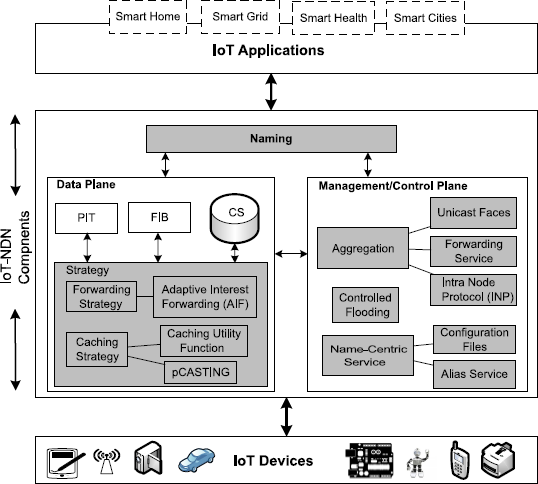
\includegraphics[width=\textwidth]{IoT-NDN_System_architecture_and_its_components.png}
%\vspace{10cm}
\centering

}






%%% Bild 2 %%%%%%%%%%%%%%%%%%%%%%%%%%%%%%%%%%%%%%%%%%%%%%%%%%%%%%%%%%%%%%%%%%%%%
\headerbox{\textsf{Figure 2}}{name=bild2, column=3, span=2, below=bild1}{
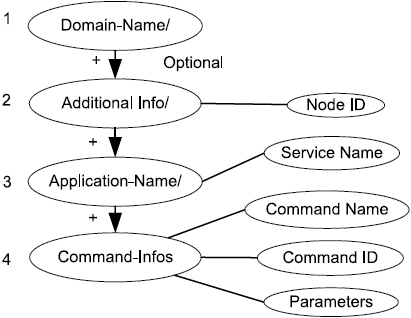
\includegraphics[width=\textwidth]{Name_Structure_of_the_suggested_Approach.png}
%\vspace{10cm}
\centering

}



%%% Bild 3 %%%%%%%%%%%%%%%%%%%%%%%%%%%%%%%%%%%%%%%%%%%%%%%%%%%%%%%%%%%%%%%%%%%%%

%\headerbox{\textsf{Bild 3}}{name=bild3, column=3, span=2, below=bild2, above=bottom}{
%	\vspace{3cm}
%\centering
%}

%%% IV. Abschnitt %%%%%%%%%%%%%%%%%%%%%%%%%%%%%%%%%%%%%%%%%%%%%%%%%%%%%%%%%%%%%%%%%%%%%
\headerbox{\textsf{Conclusion}}{name=abschnitt4, column=3, span=2, below=bild2}{
	
	\vspace{0.5em}
	IoT-NDN solves the problems of data aggregation, naming scalability, 
	and the handling of IoT devices.
	\begin{itemize}
	\item Data aggregation: by combining similar data, data aggregation is achieved.
	\item Naming scalability: devices don't need IP addresses because the data is addressed, not the device.
	\item Resource-constrained devices: having smart in-network caching, a reduced overhead, and robust pathfinding mitigate the device’s shortcomings.
	\end{itemize}
	\vspace{0.5em}
}


%%% References %%%%%%%%%%%%%%%%%%%%%%%%%%%%%%%%%%%%%%%%%%%%%%%%%%%%%%%%%%%%%%%%%%%%%
\headerbox{\textsf{References}}{name=references, column=3, span=2, above=bottom, below=abschnitt4}{
\renewcommand{\refname}{}
\begin{thebibliography}{00}
\begin{footnotesize}
\bibitem{b1} T. Teubler, M. A. M. Hail, and H. Hellbr¨uck, “A solution for the
naming problem for name-centric services,” in Wired/Wireless Internet
Communications, A. Mellouk, S. Fowler, S. Hoceini, and B. Daachi, Eds.
Cham: Springer International Publishing, 2014, pp. 214–227.
\bibitem{b2} M. A. Heil, "IoT-NDN: An IoT Architecture via Named Data
Netwoking (NDN)" "in" Software Embedded System Department
Euroimmun AG, a PerkinElmer Company
\bibitem{b3} T. Teubler, M. A. M. Hail, and H. Hellbr¨uck, “Efficient Data Aggregation
with CCNx in Wireless Sensor Networks,” in 19th EUNICE Workshop
on Advances in Communication Networking (EUNICE 2013), Germany.
\end{footnotesize}
\end{thebibliography}

 % \begin{small}
  %\renewcommand{\refname}{\vspace{-0.8em}}
  %\setlength{\parskip}{0cm}
 % \setlength{\bibsep}{0cm}
 % \bibliographystyle{unsrt}
  %\bibliography{}

%[1] T. Teubler, M. A. M. Hail, and H. Hellbr¨uck, “A solution for the
%naming problem for name-centric services,” in Wired/Wireless Internet
%Communications, A. Mellouk, S. Fowler, S. Hoceini, and B. Daachi, Eds.
%Cham: Springer International Publishing, 2014, pp. 214–227.

%[2] M. A. Heil, ”IoT-NDN: An IoT Architecture via Named Data Netwoking
%(NDN)” ”in” Software Embedded System Department Euroimmun AG,
%a PerkinElmer Company

%[3] T. Teubler, M. A. M. Hail, and H. Hellbr¨uck, “Efficient Data Aggregation
%with CCNx in Wireless Sensor Networks,” in 19th EUNICE Workshop on
%Advances in Communication Networking (EUNICE 2013), Germany.



  %\end{small}
}

\end{poster}

\end{document}